\documentclass[aspectratio=169]{beamer}
% \pdfpagewidth=1920bp
% \pdfpageheight=1080bp

% No navigation or headline
\setbeamertemplate{navigation symbols}{}
\setbeamertemplate{headline}{}
\setbeamertemplate{bibliography item}{}
\usepackage{xcolor}
\usepackage{enumitem}
\setlist{nosep} % Compact lists
\usepackage{tikz}
\usepackage{hyperref}
\usepackage{graphicx}
\graphicspath{{assets/}}

% --- Biblatex setup ---
\usepackage[
  backend=biber,
  style=keynote,      % <-- Your custom .bbx/.cbx style must be in TEXINPUTS or project folder
  citestyle=keynote,
  maxbibnames=1,
  uniquename=false,
  sorting=none
]{biblatex}
\addbibresource{references.bib}

% Reference formatting
\renewcommand*{\bibfont}{\fontsize{5}{6}\selectfont}
\newcommand{\bottomleftrefs}{%
  \begin{tikzpicture}[remember picture,overlay]
    \node[anchor=south west, xshift=1pt, yshift=1pt] at (current page.south west) {%
      \parbox{0.7\linewidth}{
        \setlength{\bibitemsep}{0pt plus 0.3ex}
        \printbibliography[heading=none]
      }
    };
  \end{tikzpicture}%
}

% Custom footline
\setbeamertemplate{footline}{%
  \leavevmode%
  \begin{minipage}[b]{0.70\paperwidth}
    \vspace{0.2em}
    {\fontsize{8}{10}\selectfont \textsf{\ifdefined\slidebib \slidebib \fi}}
  \end{minipage}%
  \hfill
  \begin{minipage}[b]{0.28\paperwidth}
    \vspace{0.2em}
    \raggedleft
    {\fontsize{9}{11}\selectfont \textrm{\textcopyright~\the\year~\insertauthor}}
  \end{minipage}%
}

\newcommand{\slidebib}{}

% Metadata (replace with your information)
\title[]{Diffusion Model Track}
\subtitle{Latest Backbone in Image Synthesis}
\author[author]{Sakura}
% \institute[institute]{institute}
\date{2025/06/16\\\small\href{mailto:bili_sakura@zju.edu.cn}{bili\_sakura@zju.edu.cn}}

\begin{document}

\begin{frame}
  \begin{minipage}{0.68\linewidth}
    \titlepage
  \end{minipage}%
  \hfill
  \begin{minipage}{0.30\linewidth}
    \centering
    
\includegraphics[width=0.9\linewidth]{profile_new.jpeg}
  \end{minipage}
\end{frame}

% Place your slides here:
% \begin{refsection}
%   \begin{frame}{Image Classification: Overview}
%     \begin{figure}
%       \centering
%       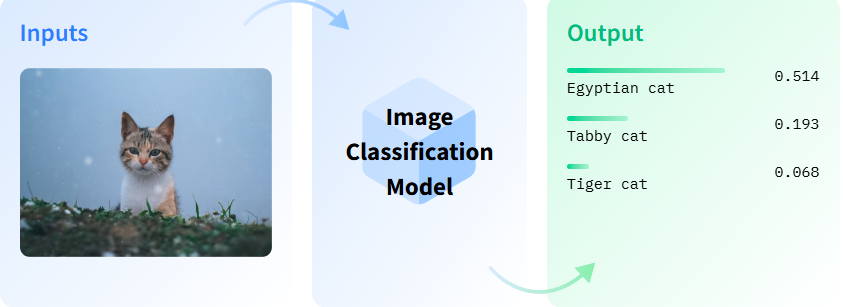
\includegraphics[height=0.6\textheight]{image_classification_idea.png}
%       \caption{\scriptsize Overview of image classification.\\\textit{Image source: Hugging Face tutorial}}
%     \end{figure}
%     \bottomleftrefs
%   \end{frame}
% \end{refsection}

\begin{refsection}
  \begin{frame}{Background: Image Classification with Deep Learning}
    \begin{figure}
      \centering
      \begin{minipage}{0.48\linewidth}
        \centering
        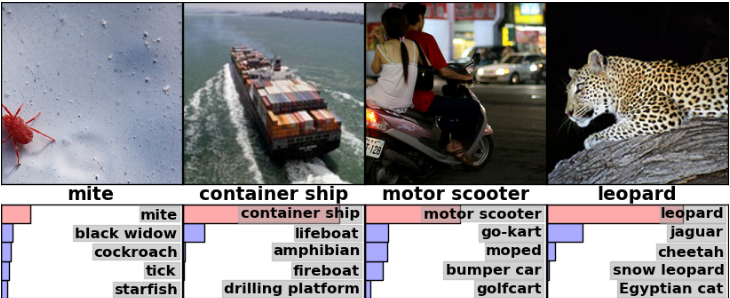
\includegraphics[width=\linewidth]{imagenet2.png}
      \end{minipage}\hfill
      \begin{minipage}{0.48\linewidth}
        \centering
        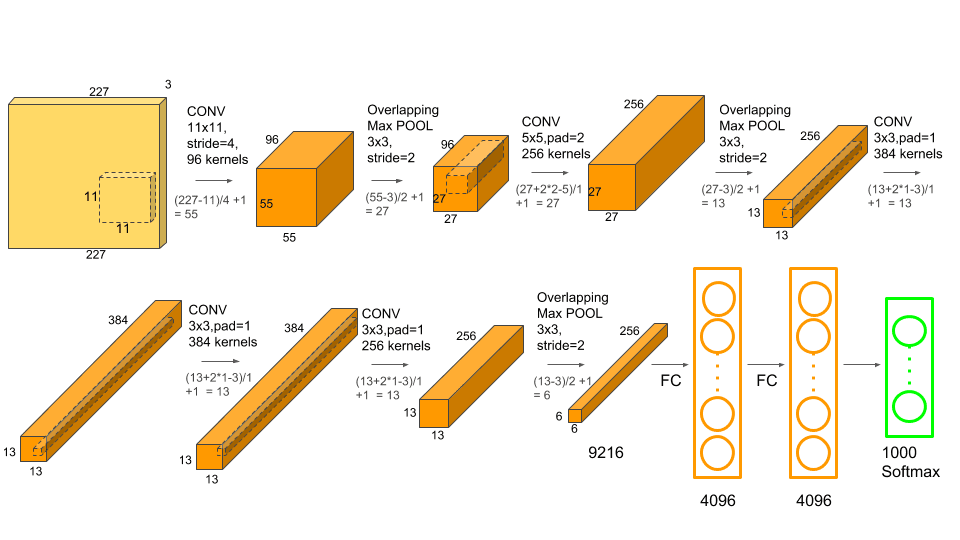
\includegraphics[width=\linewidth]{alexnet.png}
      \end{minipage}
      \caption[]{\scriptsize Left: AlexNet on ILSVRC-2010~\parencite{imagenet2010challenge} \quad Right: Architecture of AlexNet~\parencite{krizhevskyImageNetClassificationDeep2012}.}
    \end{figure}
    \bottomleftrefs
  \end{frame}
\end{refsection}

\begin{refsection}
  \begin{frame}{Architecture Evolution of Image Classification}
    \begin{minipage}{0.48\linewidth}
      {\small
      \begin{itemize}
        % \item \textbf{2012: AlexNet} \\
        % \parencite{krizhevskyImageNetClassificationDeep2012}
        % \item \textbf{2016: ResNet} \\
        % \parencite{heDeepResidualLearning2016}
        \item \textbf{2012: AlexNet}, \textbf{2016: ResNet} \\
        \item \textbf{2021: ViT} \\
        \parencite{dosovitskiyImageWorth16x162020}
        \item \textbf{2021: Swin Transformer} \\
        \parencite{liuSwinTransformerHierarchical2021}
        \item \textbf{2021: CLIP-ViT} \\
        \parencite{radfordLearningTransferableVisual2021}
        \item \textbf{2022: MAE-ViT} \\
        \parencite{heMaskedAutoencodersAre2022}
        \item \textbf{2022: CoCa-ViT} \\
        \parencite{yuCoCaContrastiveCaptioners2022}
      \end{itemize}
      }
    \end{minipage}%
    \hfill
    \begin{minipage}{0.48\linewidth}
      \centering
      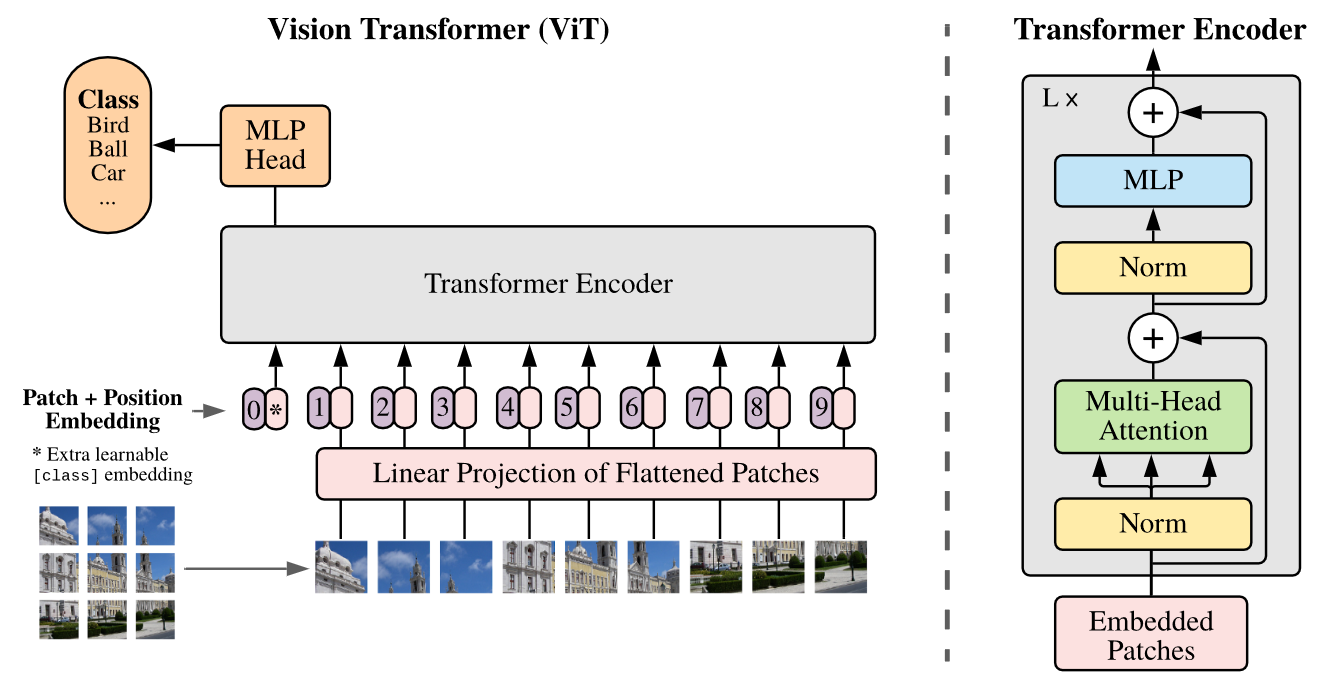
\includegraphics[width=0.95\linewidth]{vit.png}
      \scriptsize Overview of Vision Transformer\\\parencite{dosovitskiyImageWorth16x162020}.
    \end{minipage}
    \bottomleftrefs
  \end{frame}
\end{refsection}

\end{document}
